%
% Copyright (c) 2001-2005,2009 LAAS/CNRS                   --  Sat Nov  3 2001
% All rights reserved.                                     Anthony Mallet
%
% This document is a translation of the French documentation of GenoM,
% originally written by Sara Fleury and Matthieu Herrb.
%
% Redistribution  and  use in source   and binary forms,  with or without
% modification, are permitted provided that  the following conditions are
% met:
%
%   1. Redistributions  of  source code must  retain  the above copyright
%      notice, this list of conditions and the following disclaimer.
%   2. Redistributions in binary form must  reproduce the above copyright
%      notice,  this list of  conditions and  the following disclaimer in
%      the  documentation   and/or  other  materials   provided with  the
%      distribution.
%
% THIS SOFTWARE IS PROVIDED BY THE  AUTHOR AND CONTRIBUTORS ``AS IS'' AND
% ANY  EXPRESS OR IMPLIED WARRANTIES, INCLUDING,  BUT NOT LIMITED TO, THE
% IMPLIED WARRANTIES   OF MERCHANTABILITY AND  FITNESS  FOR  A PARTICULAR
% PURPOSE ARE DISCLAIMED.  IN NO  EVENT SHALL THE AUTHOR OR  CONTRIBUTORS
% BE LIABLE FOR ANY DIRECT, INDIRECT,  INCIDENTAL, SPECIAL, EXEMPLARY, OR
% CONSEQUENTIAL DAMAGES (INCLUDING,  BUT  NOT LIMITED TO, PROCUREMENT  OF
% SUBSTITUTE  GOODS OR SERVICES;  LOSS   OF  USE,  DATA, OR PROFITS;   OR
% BUSINESS  INTERRUPTION) HOWEVER CAUSED AND  ON ANY THEORY OF LIABILITY,
% WHETHER IN CONTRACT, STRICT LIABILITY, OR TORT (INCLUDING NEGLIGENCE OR
% OTHERWISE) ARISING IN ANY WAY OUT OF THE  USE OF THIS SOFTWARE, EVEN IF
% ADVISED OF THE POSSIBILITY OF SUCH DAMAGE.
%
% $Id$
%

Codels are \texttt{C} functions (at this time) that interface a module and
your algorithms: the module executes the codels, which, in turn, execute
your   own functions. In   particular,  codels can retrieve  the requests
parameters,  map them into useful data  for your functions, and then call
these functions.

% =======================================================================
\section{Different kinds of codels}

% -----------------------------------------------------------------------
\subsection{Codels associated to requests}

Sending a request to a module ends up in executing the code of the codels
associated to the request. Two types of codels can be distinguished:

\begin{itemize}
\item \textbf{control codels} (defined with \texttt{codel\_control}) are
executed by the control task. They are essentially  used for checking the
validity    of the input parameters of    the  request, just before these
parameters are actually written into the fIDS.

\item \textbf{execution codels} (defined with \texttt{codel\_main*}) are
executed by  an execution task  and  represent the actual  action of  the
service.    Their execution  create   an  activity,   which lasts   until
completion  of  the service.   These  codels  exist   only for  execution
requests.
\end{itemize}

The parameters of the \texttt{C} functions associated to  the codels are the
\texttt{ input} and \texttt{output} structures  of  the request. The input data
can thus be passed to your functions, and you can  write the results into
the output structure.


% -----------------------------------------------------------------------
\subsection{Codels associated to execution tasks}

Three codels can be optionally defined for each execution task:

\begin{itemize}
\item \textbf{Initialization codel} (\texttt{codel\_task\_start}). This codel is
executed  only once, when  the  execution task   is initialized and  just
before it starts serving requests.  One can use  this codel to initialize
the fIDS, and set default values to parameters.

\item \textbf{Termination codel} (\texttt{codel\_task\_end}). This codel is
executed by the execution task upon destruction of the module, just after
it has stopped serving requests.

\item \textbf{Permanent codel} (\texttt{codel\_task\_main}). This codel is executed
each  time  the task  wakes  up (therefore  periodically  if  the task is
periodic). This codel creates a permanent activity.
\end{itemize}


% =======================================================================
\section{Simple examples of codels}

% -----------------------------------------------------------------------
\subsection{Example of control codel}
\label{ssec|control|ex}

Control codels are used  to check the  validity of input parameters  of a
control  or  an execution request.    They can prevent entering erroneous
values  into the fIDS. For execution  requests, they can  also check that
the  module  is in   an adequate  state before  executing  the  requested
service.

Control codels take the input parameter of the  request as input and must
return either \texttt{OK} if the parameter is valid, or \texttt{ERROR} if it is
not. Warning: in the latter case, you must have defined an error code and
you must set it before returning \texttt{ERROR}.

If the  codel returns \\texttt{OK}, the  input parameter  is copied into the
fIDS and the execution  continues. If the  codel returns \texttt{ERROR}, the
parameter is not copied into the fIDS and the final reply is sent back to
the client, along with the report which has been set by the codel. For an
execution  request,  the  activity is  not  started.   The error code  is
fundamental: if it is  not  set, the client   will have no idea  of  what
happened.

As an example, here  is the control  codel \texttt{demoSetSpeedCntrl} of  the
request \texttt{SetSpeed} of the module \\texttt{demo}.  This request expects a
speed as input (structure \texttt{DEMO\_SPEED}).  Therefore, the codel takes
a pointer   to  this structure as  first  parameter.   The structure 
\texttt{DEMO\_STR}  is   defined    in  the    file  \\texttt{demoStruct.h}    (see
chapter~\ref{cha|session}).

\begin{center}\begin{cartouche}\small\begin{verbatim}
STATUS
demoSetSpeedCntrl(DEMO_SPEED *speed, int *report)
{
   /* Refuse *speed if the value is erroneous */
   if (*speed != DEMO_SLOW && *speed != DEMO_FAST) {
        *report = S_demo_INVALID_SPEED;
        return ERROR;
   }
   /* Parameter is valid: it will be entered into the fIDS */
   return OK;
}
\end{verbatim}\end{cartouche}\end{center}

% -----------------------------------------------------------------------
\subsection{Example of execution codel}

Execution  codels are always associated  to   an execution request.  They
perform the actual actions of the service.

For this first example, we will write a request  that compute the norm of
a 2-dimensional vector. The standard math library already has such a
function:

\begin{center}\begin{cartouche}\small\begin{verbatim}
double
hypot(double x, double y);
\end{verbatim}\end{cartouche}\end{center}

What we have to do now  is to add  to the module  a request which we call
\emph{Hypot}. An execution codel will do  the actual computation, and call
\texttt{hypot()}. The input parameter will be a structure which will contain
two members, \texttt{x} and \texttt{y}: we call it \texttt{DEMO\_VECTOR\_STR}. The
output parameter is a single \emph{double}.

In the file \texttt{demo.gen}, we write:

\begin{center}\begin{cartouche}\small\begin{verbatim}
/* fIDS declaration */
typedef struct DEMO_STR {
   DEMO_STATE_STR     state;           /* Current state */
   DEMO_SPEED         speedRef;        /* Speed reference */
   DEMO_VECTOR_STR    vector;
   double             norm;
   ...
};

/* Hypot request */
request Hypot {
   doc:                   "compute sqrt(x*x+y*y)";
   type:                  exec;                /* execution request */

   input:                 vector::vector;      /* vector (x, y) */
   input_info:                                 /* default values and */
      0.0::"X coordinate",                     /* description of */
      0.0::"Y coordinate";                     /* parameters */
   
   output:                norm::norm;          /* norm (result) */
   codel_main:            demoHypotExec;       /* execution codel */
   exec_task:             MotionTask;          /* execution task */
   interrupt_activity:    Hypot;               /* incompatibilities */
};
\end{verbatim}\end{cartouche}\end{center}

In the file \texttt{demoMotionTaskCodels.c}, which contains all the codels
for this task, we write the \texttt{demoHypotExec} codel:

\begin{center}\begin{cartouche}\small\begin{verbatim}
ACTIVITY_EVENT
demoHypotExec(DEMO_VECTOR_STR *vector, double *norm, int *report)
{
   *norm = hypot(vecteur->x, vecteur->y);
   return ETHER;
}
\end{verbatim}\end{cartouche}\end{center}

The \\texttt{return  ETHER} statement tells   \GenoM\ that  the  activity is
terminated: the client will  get the final  reply. We will see  later the
other values that can be returned at the end of an execution codel.

The next  step is to  compile the   module,  and link   it with the  
\texttt{hypot()} function.  In  this  case, \\texttt{hypot} is   a function of   the
standard library, so there's nothing special  to do.  But it the function
were a function of your own, defined in a non-standard library, you would
have to edit the Makefiles and complete the variables:

\begin{itemize}
\item \texttt{CPPFLAGS} for the path to the headers of your library.
\item \texttt{LIBS} for the path to the library itself.
\end{itemize}

Here is what it could look like with our example and the Makefile in the
\texttt{codels/} directory:

\begin{center}\begin{cartouche}\small\begin{verbatim}
[...]
CPPFLAGS += -I$(DEMO) -I$(DEMO)/server -I$(DIRUNIX)  -I$(DIRGENOM)
CPPFLAGS += -I/usr/include
[...]
LIBS = /usr/lib/libm.a
\end{verbatim}\end{cartouche}\end{center}
%$

If your external functions  were defined in a  \texttt{C}  file in the  
\texttt{codel/} directory (instead of  in an external  library), you would simply
add this file to the   list  of files to  be   compiled into the   codels
library:

\begin{center}\begin{cartouche}\small\begin{verbatim}
[...]
SRCS = \
        demoCntrlTaskCodels.c \
        demoMotionTaskCodels.c
SRCS += hypot.c
[...]
\end{verbatim}\end{cartouche}\end{center}

This simple example showed how to integrate  your algorithms into codels.
The sections~\ref{sec|codels|split} page~\pageref{sec|codels|split} and
\ref{sec|codels|writing} page~\pageref{sec|codels|writing} will present
more complex examples.


% =======================================================================
\section{Codel files and compilation}

\subsection{Splitting codels into several files}

To help you   write the  codels, the \\texttt{-i}  option of  \\texttt{genom}
generates empty templates in the \\texttt{codels/} directory. Then, you just
have to complete the templates.

\emph{Note}  that if you use the  \texttt{-i} option  and those files already
exist, \texttt{genom} asks for confirmation before  overwriting any file. It
is not possible to  fuse locally modified  templates with fresh new ones.
However, the   templates are always generated  in  the  \texttt{.genom/codels/}
directory, so  that  you can fuse   parts together by  yourself. The 
\texttt{genom-mode} can help you to do this: see chapter~\ref{cha|edit}.

By default, there is one codel file per task.  Control codels are grouped
in the  source file  \texttt{demoCntrlTaskFunc.c}  and execution  codels are
grouped  in the the source  file \texttt{demo<Exec  Task>Func.c}, where 
\texttt{<Exec Task>} is the name of the execution task for those codels.

You are    free  to define   additional  files,  or  change  the  initial
organization.  Be sure you update the  \texttt{SRC} variable in the Makefile
to reflect your changes.


\subsection{Makefiles}

Several \\texttt{Makefile} are generated   by \texttt{genom}.  By default, they
compile your codels  files, and perform the  link edition with the module
server (\texttt{demoServer.a} for Unix).

Each file  is compiled in the \\texttt{\$\{TARGET\}} subdirectory. For unix,
the compilation  produces the executable \texttt{demo}.

You can change the standard Makefiles to suit your needs. In particular,
you can:

\begin{itemize}
\item add files to the \texttt{SRC} list.
\item add libraries to the \texttt{LIBS} list.
\item add compilation flags such as \texttt{-I} or \texttt{-D} to the  variable
\texttt{CPPFLAGS}.
\end{itemize}


% =======================================================================
\section{Accessing the IDS}

You can access   this  structure from a  codel  at  any time.   A  mutual
exclusion lock protects the structure against concurrent accesses.

\subsection{The fIDS}

The macro \texttt{SDI\_F}  defined in the \texttt{server/<module>Header.h} header
represent a pointer to the fIDS of the module.

\emph{Warning:} 
 You should not read parameters
of  a  request  directly  from the  fIDS,  but only from the codel
function parameters.

Indeed, the   \texttt{input}  and \\texttt{output} parameters  of   the
requests  can  be those  of simultaneous activities  (if  the  request is
compatible with  itself).  In that case, these  parameters \emph{are not}
pointers to members of  the fIDS structure declared in  the module.  Each
activity  must have  its own  set  of  parameters, and \GenoM\  generates
arrays for that case. The member you have defined in the \emph{fIDS} still
exists, but is not used.

\subsection{The cIDS}

The cIDS contains various parameters of the module (period, poster names,
clients ids, \ldots) and its current  state (activities, \ldots). You can
read  the members  of this  structure thanks   to macros  defined in 
\texttt{server/<module>Header.h}.

This cIDS is also exported in the control poster of the module.

Warning: the control poster belongs to the control task of the module.
It updates this poster every time it wakes up, ie, when it receives
a request or when an activity is over. However, the activity state
transitions, executed by the execution tasks, are usualy much more
frequent. Thus, the control poster is not updated in real time.


Here is a non-exhaustive list, for a module \\texttt{pilo} client of another
module \texttt{loco} and with an execution task \texttt{Motion} which updates a
poster \texttt{Ref}:

\bigbreak

{\small\begin{tabularx}{0.8\linewidth}{|l|X|}
\hline
name & value\\
\hline
\tt PILO\_MOTIONTASK\_NUM    & Id of the exec. task \texttt{MotionTask}\\
\tt PILO\_REF\_POSTER\_ID    & Poster \texttt{Ref} Id\\
\tt PILO\_MOTION\_LOCO\_CLIENT\_ID & Client id for \texttt{loco}\\
\tt CURRENT\_ACTIVITY\_NUM($i^*$) & Current activity number\\
\tt EXEC\_TASK\_PERIOD($i^*$) & Execution task period (seconds)\\
\hline
\end{tabularx}}

($*$)  $i$ is   the  id  of  the    execution  task, for   instance  
\texttt{PILO\_MOTIONTASK\_NUM}.


% =======================================================================
\section{Reports}

In real situations, every action can fail. On a machine which
interacts with  its environment, it is \emph{necessary} to think of every
such abnormal situation, in order to protect the whole system. In case of
an execution error,  it  is necessary to \emph{i.} restore a sane  state
locally, to be able to restart another  execution and \emph{ii.}  report a
precise information   to the  client so  that   it can   take appropriate
decisions.

The list of abnormal situations is defined with the field \texttt{fail\_reports}
of every   request.  These   are strings,   wich are   meant to be  human
readable:       for      instance  \\texttt{INVALID\_PARAMETERS},   
\texttt{POSTER\_NOT\_FOUND}, \texttt{NOT\_ENOUGH\_MEMORY},   \texttt{IMPORTANT\_DRIFT},
\texttt{CASE\_NOT\_MANAGED},\\ \texttt{SOLUTION\_NOT\_FOUND}, \ldots

Reports must be precise:  avoid strings such  as \texttt{ERROR}. However, it
is not necessary to recall the name  of the request:  the client knows it
already.  Thus, a  report \\texttt{INVALID\_PARAMETERS}   could be used  for
several requests without loss of information.

Modules must  also   restore  themselves into  a  sane  state  and handle
correctly future   requests.   For  instance, in  the   case  of  a  
\texttt{NOT\_ENOUGH\_MEMORY}, the module should free every unused memory in order
to be able to process  less demanding requests.  If  the failure is  such
that the module cannot restore a sane sate, it should put itself into the
\texttt{ZOMBIE} state and wait for a human debugger.


\subsection{Numerical values of reports}

Reports which  are declared in the \\texttt{fail\_reports} field are mapped into
32 bits integers using the VxWorks convention:

The name of this integer is build as follow: \texttt{S\_<source>\_<report>},
where \texttt{<source>} is the name of the module or the library which defines
the      \\texttt{<report>}     string.    For       instance:     
\texttt{S\_demo\_INVALID\_PARAMETER}.

The numerical value is computed as follow:
\begin{itemize}
\item the 16 highest significative bits encode the id of the task or
the  library which  defines the report.   This  number is  the  id of the
module  $N$.

\item the 16 lowest significative bits encode the id of the report
inside the module, and is computed by \GenoM.
\end{itemize}

Error codes are stored in the file \texttt{server/<module>Error.h}.



% =======================================================================
\section{Updating posters}

Posters which are  declared as \texttt{user}  must be updated by the codels.
There are several ways to do so: depending on the type of poster, you can
use  functions of    the      poster  library \\texttt{posterLib}      (see
appendix~\ref{anx|posters}) or   the function  generated by \GenoM\  (see
below).  The function \texttt{posterWrite} is of particular interrest:

\bigbreak
\texttt{int posterWrite(POSTER\_ID posterId, int offset, char *buf, int nbytes)}
\bigbreak

\texttt{posterId} is the poster id: e.g. \texttt{PILO\_REF\_POSTER\_ID} for the
poster \texttt{Ref} in  module \\texttt{pilo}.   \texttt{posterWrite} writes  
\texttt{nbytes} from buffer \texttt{buf} in the poster structure, starting at offset
\texttt{offset}.  It returns the  number of bytes actually written, normally
\texttt{nbytes}.

\bigbreak

Consider the example  of poster \\texttt{Mobile} in module \\texttt{demo}. Its
structure is:

\begin{center}\begin{cartouche}\small\begin{verbatim}
typedef struct DEMO_MOBILE_POSTER_STR {
  DEMO_STATE_STR state;
  double ref;
} DEMO_MOBILE_POSTER_STR;
\end{verbatim}\end{cartouche}\end{center}
\label{typedef|demomobile}

Example 1: you update the \texttt{ref} member. Since it is not at the
beginning of the poster, you must compute the offset:

\begin{center}\begin{cartouche}\small\begin{verbatim}
   DEMO_MOBILE_POSTER_STR *mobile;
   int offset;
   double ref;
   ...
   offset = (char *)(&mobile->ref) - (char *)(&mobile);
   posterWrite(DEMO_MOBILE_POSTER_ID, offset, &ref, sizeof(ref));
\end{verbatim}\end{cartouche}\end{center}

Example 2:  \GenoM\ produces a  function that  do the  same as  the above
example:

\begin{center}\begin{cartouche}\small\begin{verbatim}
   double ref;
   ...
   if (demoMobileRefPosterWrite(DEMO_MOBILE_POSTER_ID, &ref) == ERROR) {
        /* stop ... */
   }
   ...
\end{verbatim}\end{cartouche}\end{center}

\bigbreak

Another more practical  method consists in getting  the actual address of
the poster   structure.   This is done thanks    to the  \texttt{posterAddr}
function. This function returns a pointer to the structure of the poster,
and you can  write into it directly. Be  sure to protect writings to  the
poster with \texttt{posterTake} before    writing anything in it and    
\texttt{posterGive} once you are done.

The three functions take one  parameter: the poster id. \texttt{posterTake}
takes another  argument:  \texttt{POSTER\_WRITE} or  \texttt{POSTER\_READ}, for
accessing the poster in write or read mode.

\begin{center}\begin{cartouche}\small\begin{verbatim}
    static DEMO_STATE_POSTER_STR *addrPosterMotion = NULL;

    /* Get the poster address */
    addrPosterMotion = posterAddr(DEMO_STATE_POSTER_ID);
    if (addrPosterMotion == NULL) {
       *report = errnoGet();
       return ERROR;
    }

    /* Update the poster */
    posterTake(DEMO_STATE_POSTER_ID, POSTER_WRITE);
    addrPosterMotion->state.speed = state.speed;
    posterGive(DEMO_STATE_POSTER_ID);
\end{verbatim}\end{cartouche}\end{center}


% =======================================================================
\section{Splitting algorithms into codels}
\label{sec|codels|split}

As   we have   already  mentioned,  algorithms   must  be integrated into
codels. In the simple example presented  in the beginning of the chapter,
the  \texttt{hypot} function  was put in a   single codel.  For more complex
algorithms, it will be necessary to split the functions call into several
codels. You will have to write the succession of codel calls.

The choice  of the number of  codels is generally  not unique.  But it is
important to keep in mind that a codel  is the \emph{smallest} entity that
a module can handle. In particular, a  codel cannot be \emph{interrupted}:
during  its execution the   module cannot do   anything else. The way you
split your algorithms will thus determine the latency of the module.

Consider  the two most  common classes of   codels: periodical codels and
aperiodical codels.

\subsection{Periodical codels}

For periodical codels (servoing, monitoring, filtering, \ldots), the same
function must be called periodically. To do so, an execution request will
be associated  to  a periodical  execution task  and  the  codel will  be
invoked at each period.

Typically, this codel  will be the \emph{execution codel} of the  request
(\\texttt{codel\_main}).  To let   the    execution task call   the  codel
periodically, the latter must let the task know that  the activity is not
finished  when the codel  returns.  This is done  by returning \texttt{EXEC}
instead  of \texttt{ETHER}.  The activity stays  in the state \texttt{EXEC} and
the execution codel will be called at the next task's wake up.

Consider request \texttt{Monitor},   which monitorates the position   of the
mobile and  throw an  alert when it   has the requested value, say,  
\texttt{myPos}.  The  execution codel  \\texttt{demoMonitorExec} (see below)  is invoked
(\texttt{return EXEC;}) until the position \texttt{myPos}  has not been reached
with the \texttt{DEMO\_THRESHOLD} precision. Once  this position is reached,
the activity ends (\texttt{return  ETHER;}) and the  final reply is sent  to
the client.

\begin{center}\begin{cartouche}\small\begin{verbatim}
ACTIVITY_EVENT
demoMonitorExec(double *monPos, double *pos, int *report)
{
   /* Get the current position */
   *pos = SDI_F->state.position;

   /* Test if we are in the monitored zone */
   if (fabs(*monPos - *pos) > DEMO_THRESHOLD) {

      /* if not, we continue with the same codel */
      return EXEC;
   }

   /* The mobile is in the goal area: end the activity */
   return ETHER;
}
\end{verbatim}\end{cartouche}\end{center}

In this example,   we used only  one execution  codel, which  was invoked
periodically.

If an algorithm had required an  initialization step (e.g.  for a sensor,
a variable, starting another service, \ldots), this  would have been done
thanks to the \emph{start} codel (\texttt{codel\_start}).  This codel
corresponds to the \texttt{START} state, and  is always executed first if it
is  defined. At the  end  of this codel,  we  would \texttt{return EXEC;} to
switch to  the \\texttt{EXEC} state, or   \texttt{ETHER} if   we  want to  stop
everything.

Similarily, a termination phasis   would be defined   thanks to the  {\em
termination codel} (the \texttt{codel\_end} field) associated to the
\texttt{END} state. To indicate, at the end of  the execution codel, that we
want to go through this  termination state, we just  have to \\texttt{return
END;} instead of \texttt{ETHER}.


\subsection{Aperiodical codels}

In  the case of  an aperiodical codel (e.g.   a trajectory planning), the
request associated  to the codel  will be  associated to  an  aperiodical
execution task. The codel  could be made up of  only one part, but if its
execution took  a while,  it  would be advised  to  split it into several
atomic pieces.  You can then use the different states as mentioned in the
previous section to glue pieces together.


\subsection{Interrupting a codel}

An activity that  goes through several  codels (or  several times through
the  same codel), can  be  interrupted.  (as  we already  mentioned it, a
single codel cannot be interrupted). When  this occurs, the activity goes
into the  \texttt{INTER}rupted  state,  and the  \\texttt{codel\_inter}
codel is executed.  By default, there is  no such codel, and the activity
goes immediatly into the \texttt{ETHER} state.

A  sudden  interruption can   sometimes  be problematic.  You  might  for
instance  want  to stabilize a dynamic   system before actually stopping,
free some memory, or stop another activity which is correlated to the one
which   is  beeing     interrupted.  In   that  case,   define    a  
\texttt{codel\_inter} codel which will handle the necessary operations.


\subsection{States and transitions of activities}

The   different  states   an  activity can   go   through  are  shown  on
figure~\ref{fig|states}. The external ring correspond to the \emph{normal}
sequencing: \\texttt{ETHER} $\rightarrow$   \texttt{START} $\rightarrow$   
\texttt{EXEC} $\rightarrow$ \texttt{END}  $\rightarrow$ \texttt{ETHER}. \texttt{START} and
\texttt{END}  states are optional.   On any transition, one  can go into the
\texttt{INTER} state.

\begin{figure}[htbp]
\centering
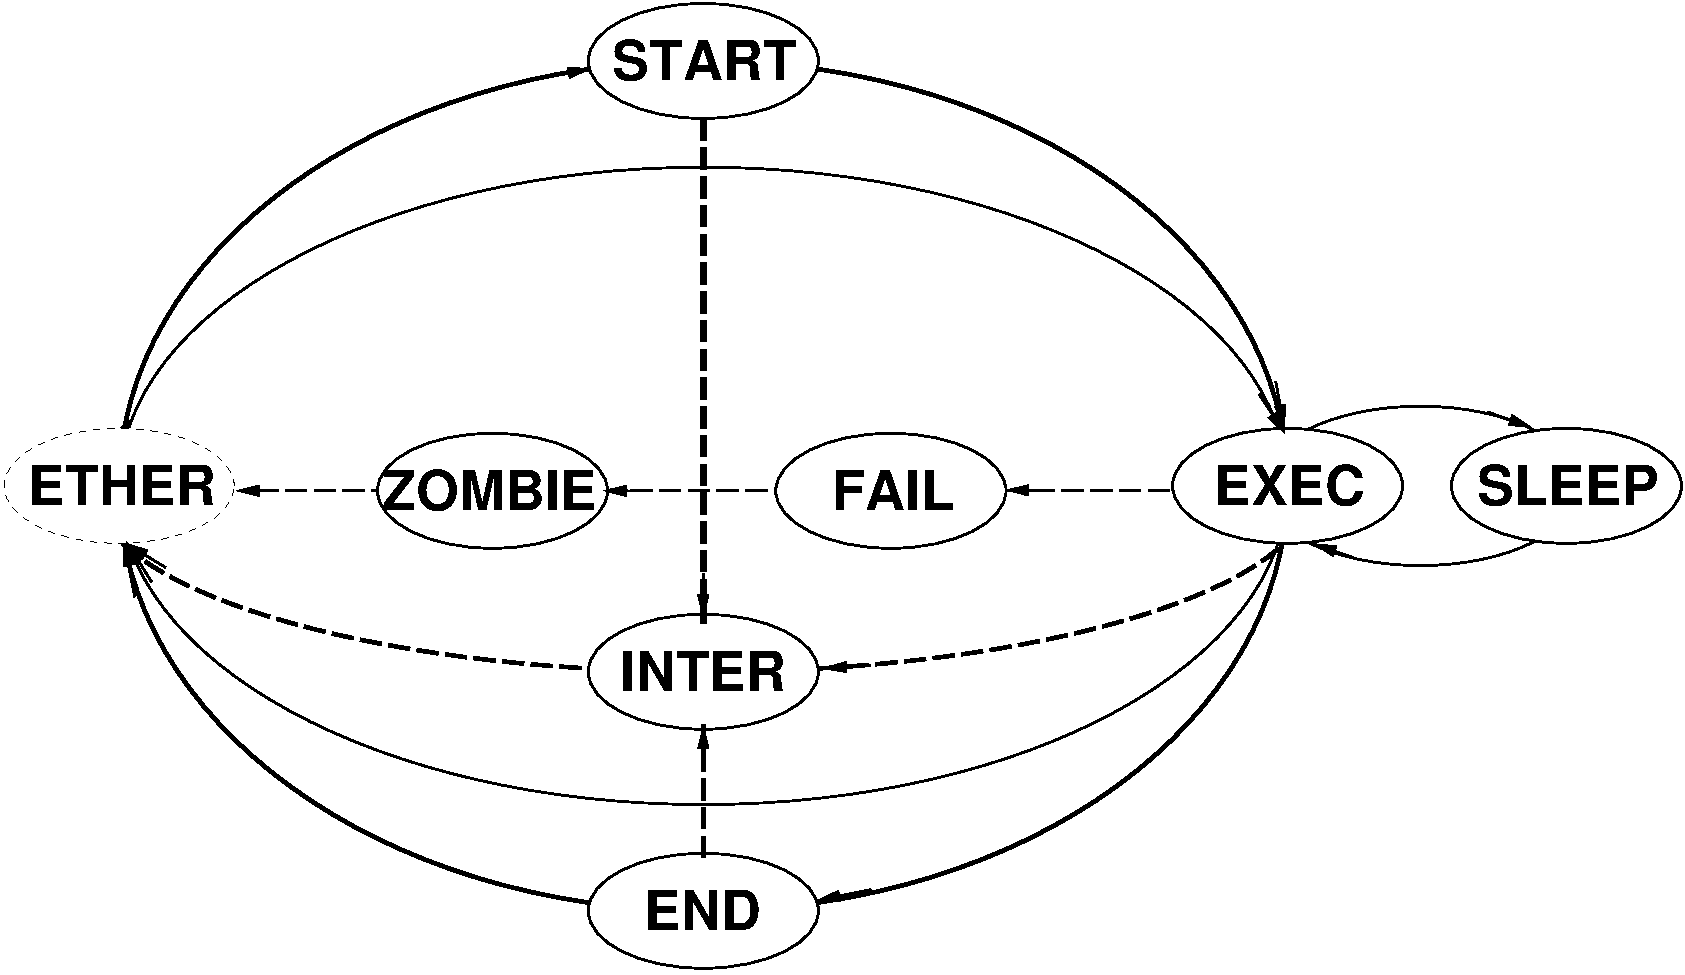
\includegraphics[width=0.8\hsize]{fig/activity-states}
\caption{States and transitions of activities.}
\label{fig|states}
\end{figure}

Note: in case of a problem, one can go into the \texttt{FAIL} state, or even
directly into the \texttt{ZOMBIE} state. The module is then frozen.

As of today, the  number of states is fixed  and  a future version  might
change this.  However, a workaround  is  still possible with the  current
version, by using internal   state   variables. The current  states   are
recalled in the following table:

\bigbreak

{\small\begin{tabularx}{0.8\linewidth}{|l||X|l|}
\hline
state 	& comments 	& codel (if defined)	  \\
\hline
\tt START  & startup state 
		& \tt codel\_start 	\\
\tt EXEC   & main execution state & \tt codel\_main  \\
\tt END    & termination state 	& \tt codel\_end \\
\tt FAIL   & failure (and module freeze) \em 
					& \tt codel\_fail \\
\hline
\tt INTER  & interruption state 
					& \tt codel\_inter  \\
\hline
\tt SLEEP     	&  suspended activity (waits an external event to go back
into  \texttt{EXEC} ) & \\
\tt ETHER    	& \em terminated activity  & \\
\tt ZOMBIE   	& \em terminated activity and frozen module & \\
\hline
\end{tabularx}}

\bigbreak

State description:

\begin{itemize}
\item \texttt{START} is the first step of the execution. If the codel is not
specified, the activity goes directly into state \texttt{EXEC}.
\end{itemize}

It is up  to you to define the   following transitions. To  do so, codels
must return one value of  the enum \\texttt{START},  \texttt{EXEC}, \\texttt{END},
\texttt{ETHER},  \texttt{FAIL}, \\texttt{ZOMBIE} or \texttt{SLEEP}, which corresponds
to the state of the same name. One does normally follow the sequence 
\texttt{START} $\rightarrow$ \\texttt{EXEC} $\rightarrow$  \\texttt{END} $\rightarrow$
\texttt{ETHER}.

\begin{itemize}
\item \texttt{EXEC}, \texttt{END} and \texttt{INTER} are decribed in the previous
sections.

\item \texttt{ETHER} indicates that the activity does not exist anymore.

\item \texttt{ZOMBIE} indicates that the activity stopped due to an abnormal
situation. The module  is then  frozen and  will not answer  any requests
anymore. A special request \texttt{Abort} let you resume the activity, which
then  goes into the  \texttt{ETHER} state. This  state can  be useful if you
want  to debug  some problem.  It   can also be  useful   if you want  to
re-synchronize two modules.

\item \texttt{FAIL} terminates the activity, just before going into 
\texttt{ZOMBIE}. The codel can do some additional cleanup.

\item \texttt{SLEEP} suspends an activity, and waits for an external event
to occur (a request,  or an \\texttt{h2evn} event). Then  it returns  to the
\texttt{EXEC} state.
\end{itemize}

The following table summarize the possible transitions, for each state:

\bigbreak

{\small\begin{tabular}{|ll||c|c|c|c|c|c|}
\cline{3-8}
\multicolumn{2}{c}{} & \multicolumn{6}{|c|}{possible transitions} \\
\hline
state & (codel) & \tt START & \tt EXEC/SLEEP & \tt END & \tt ETHER & \tt FAIL & \tt ZOMBIE \\
\hline
\tt START  & \tt (codel\_start)	& X & X & X & X & X & X \\
\tt EXEC   & \tt (codel\_main) 	&   & X & X & X & X & X \\
\tt END    & \tt (codel\_end) 	&   &   & X & X & X & X \\
\tt INTER  & \tt (codel\_inter) &   &   &   & X & X & X \\
\tt FAIL   & \tt (codel\_fail) 	&   &   &   &   & X & X \\
\hline
\end{tabular}}

Note: a termination state (\texttt{END}, \texttt{FAIL} or \texttt{INTER}) is never
interrupted.


% =======================================================================

\section{Writing the codels}
\label{sec|codels|writing}


\subsection{Control codels  \texttt{codel\_control}}

See        example            in           section~\ref{ssec|control|ex},
page~\pageref{ssec|control|ex}.

\subsection{Execution codels  \texttt{codel\_*}}

Execution  codels have 1,  2 or 3  parameters,  depending on the request.
These codels can have,  in this order and   if the corresponding  data is
defined,  a pointer to  the   input structure,  a pointer  to  the output
structure and a pointer to the report (always  defined). Codels return an
\texttt{ACTIVITY\_EVENT}, as exposed in the previous section.

Here is the \texttt{demoGotoPosition}  execution codel (\texttt{codel\_main})
of the \texttt{Goto} request of the module \texttt{demo}. This codel,
invoked periodically, controls the speed of the mobile (according to the
one specified with the \texttt{SetSpeed} request), and stops when the
requested position is reached. We suppose we have two low level functions
which control the mobile:

\begin{itemize}
\item \texttt{STATUS mobileState(double *position, double *speed)} which get
the current status of the mobile (thanks to sensors) and
\item \texttt{STATUS mobileMove(double position, double speed)} which move
the mobile to the requested position at the requested speed.
\end{itemize}

\begin{center}\begin{cartouche}\small\begin{verbatim}
ACTIVITY_EVENT
demoGotoPosition(double *goal, int *report)
{
   double remain;       /* remaining distance (m) */
   double speed;        /* requested speed (m/s) */
   double increment;    /* position change (m) */

   /* Measure current speed and position */
   if (mobileState(&(SDI_F->state.position), &(SDI_F->state.speed)) != OK) {
        *report = S_demo_MOBILE_OUT_OF_ORDER;
        return ETHER;
   }

   /* Compute the remaining distance */
   remain = *goal - SDI_F->state.position;

   /* Get the reference speed */
   if (SDI_F->speedRef == DEMO_SLOW) 
        speed = DEMO_SLOW_SPEED;
   else
        speed = DEMO_FAST_SPEED;

   /* Compute an elementary move, according to the speed and period */
   increment = speed * DEMO_MOTION_TASK_PERIOD;

   /* Are we done? */
   if (fabs(remain) < increment) {
        if (mobileMove(*goal, 0) != OK) {
            *report = S_demo_MOBILE_OUT_OF_ORDER;
            return ETHER;
        }
        return END;
   }

   /* Continue */
   if (mobileMove(SDI_F->state.position +
                      SIGN(remain) * increment, speed) != OK) {
        *report = S_demo_MOBILE_OUT_OF_ORDER;
        return ETHER;
   }
   return EXEC;
}
\end{verbatim}\end{cartouche}\end{center}

Notes:

The \texttt{SDI\_F} macro let you acces the fIDS structure.

\texttt{DEMO\_MOTION\_TASK\_PERIOD} is the period of the execution task
(stored in the cIDS).

We will see later how one can access IDSs and how reports can be used.


\subsection{Initialization codel \texttt{codel\_task\_start}}

One initialization codel can be associated to any  execution task, by the
mean of the field \\texttt{codel\_task\_start}. It is  usually used to initiliaze
the fIDS to a known state. It takes only one  parameter: a pointer to the
report.   It returns either \\texttt{OK}  or \texttt{ERROR}  (in  that case the
module does not start).

For the \texttt{demo} module,  this codel chooses  a  default speed for  the
mobile  and intializes its state.   Note  that fISD are not automatically
initialized with zeros.

The constants and default values used by a  module are usually defined in
a header file in the main directory  of the module. In  that case this is
\texttt{demoConst.h}.

\begin{center}\begin{cartouche}\small\begin{verbatim}
STATUS
demoInit(int *report)
{
  SDI_F->state.position = 0.;
  SDI_F->state.speed = 0;
  SDI_F->distRef = 0;
  SDI_F->posRef = 0;
  SDI_F->speedRef = DEMO_SLOW;

  return OK;
}
\end{verbatim}\end{cartouche}\end{center}


\subsection{Permanent activity codel \texttt{codel\_task\_main}}

A permanent activity can  be defined for  any execution task, by the mean
of the  field  \texttt{codel\_task\_main}.  It is executed  each  
time the task  wakes up. 
It is usually used to set up a  filtering function (pose computation,
sonar echos  reading, \ldots), or   a permanent  servoing activity  which
starts and stops with the module.

This codel takes only one parameter, a pointer on the report, and returns
a \texttt{STATUS} (\texttt{OK} or \texttt{ERROR}).  Be warned that  if an error is
returned, the execution task  is \emph{suspended} (it  is resumable with a
\texttt{taskResume}).

Since this activity is not associated to a  request, the report is stored
in the cIDS as well as in the control poster. Clients can read the poster
to know the status of this activity.


% =======================================================================
\section{Parallel activities and synchronization}

Execution   requests can  only  be  declared  \emph{compatible} or  {\em
incompatible} with each other. In the first case, their execution becomes
completely  independent one another.  In  the second case, they interrupt
themselves.  There are  some   intermediate  cases, where  requests  must
synchronize, or exchange  data.   Those cases are  to  be handled  by the
codels.

To  do so, it is  possible to use \emph{activity  ids}: each eactivity is
identified by a number between  $0$ and \texttt{MAX\_ACTIVITIES}$-1$. From a
codel,   the current  activity number  is    returned by the  macro  
\texttt{CURRENT\_ACTIVITY\_NUM}.

This  id can be  used  to exchange   information between activities.  For
instance, it would  be possible to  declare  a global (static) array,  of
size \\texttt{MAX\_ACTIVITIES},    in which   each  element   would  contain
information regarding each activity  (current state, order of  arrival of
the request, number of the previous and next activity, \ldots).

Consider  the following  example,  where  you wish  to \emph{concatenate}
several motion  requests  for a   mobile.  The  motion  request  must  be
compatible with  itself (because it must not  interrupt the latest motion
request)  \emph{but} the execution codel  \texttt{EXEC} must not start before
the previous request has completed.  This must be handled internally, and
the  transition \texttt{START}  $\rightarrow$  \texttt{EXEC}  of a new activity
must be  synchronized with the  transition \\texttt{EXEC} $\rightarrow$ 
\texttt{END} of the activity.

Such  a  synchronization     can  be  achieved   in     the   codel  
\texttt{codel\_start}. This codel can register new activities in a global
array, attach to them the previous activity, and  stay in the \texttt{START}
state  until the previous activity  stops. The latter information will be
registered by the codel \texttt{codel\_end}.

The following  code  proposes an  example of such   start and end codels,
along with the global data definition:


\begin{center}\begin{cartouche}\small\begin{verbatim}
/* Global array for "Motion" requests */
struct DEMO_MOTION_STR {
    ACTIVITY_EVENT state;
    int next;
} demoMotionTab[MAX_ACTIVITIES] = {ETHER, -1};

/* Latest "Motion" request sent */
static int demoMotionLast = -1; 
\end{verbatim}\end{cartouche}\end{center}

\begin{center}\begin{cartouche}\small\begin{verbatim}
/* Start codel codel_start of the "Motion" activity */
ACTIVITY_EVENT
demoMotionStart(MOTION_STR *params, int *report)
{
    int current = CURRENT_ACTIVITY_NUM(DEMO_MOTIONTASK_NUM);

    /* If that is a new activity */
    if (demoMotionTab[current].state == ETHER) {

        /* If there is an active activity: wait */
        if (demoMotionLast != -1) {
            demoMotionTab[current].state = START;
            demoMotionTab[demoMotionLast].next = current;
        }
        /* No activity: one can start immediately */
        else {
            demoMotionTab[current].state = EXEC;
        }

        /* Append ourselves to the end of the list */
        demoMotionLast = current;
    }
    return (demoMotionTab[current].state);
}
\end{verbatim}\end{cartouche}\end{center}

\begin{center}\begin{cartouche}\small\begin{verbatim}
/* Termination codel codel_end of the "Motion" activity */
ACTIVITY_EVENT
demoMotionEnd(MOTION_STR *params, int *report)
{
    int current = CURRENT_ACTIVITY_NUM(DEMO_MOTIONTASK_NUM);
    int next;

    /* Next activity number */
    next = demoMotionTab[current].next;

    if (next == -1) 
       /* If there is no next activity */
        demoMotionLast = -1;
    else
       /* Unblock next activity */
        demoMotionTab[next].state = EXEC;

    /* This activity is terminated */
    demoMotionTab[current].next = -1;
    demoMotionTab[current].state = ETHER;
    return ETHER;
}
\end{verbatim}\end{cartouche}\end{center}

Warning: if   a   synchronized activity   fails (either  because   it  is
interrupted or because of a problem), it must signal  it to other pending
activities in order to also cancel them. It will also be necessary to set
up  a way to  re-synchronize  with clients,  for  instance with a control
request.


% =======================================================================
\section{Coding advice}

\subsection{General coding rules}

A  module is designed  to be  integrated in a  complex system:  users and
maintainers are usually not the same people.  For this reason, it is very
important to respect a few coding rules.

\begin{itemize}
\item Split programs into functions and files of a reasonable size;

\item Prototype functions;

\item Comment your code while you are writing it: 
   \begin{itemize}
   \item A comment for each function which documents the purpose and the
	 limitations you are aware of.
   \item A comment for an average of 3 or 4 lines of code.
   \end{itemize}

\item Avoid global variables;

\item Avoid magic numbers (use constants and \texttt{\#define}).

\item Choose a uniform style, and follow it. For instance, the VxWorks
      programmers manual recommends the use of 
all uppercased  words, separated by underscores  for constants (e.g. 
\texttt{DEMO\_SPEED}) and lowercase words, with a first uppercase letter for each
word but the first (e.g. \texttt{controlSpeed}) for symbols;

\item Prefix all exported symbols (types, constants, functions, \ldots)
with e.g. the module name;

\item Use explicit names. Avoid short names such as \texttt{i}, \texttt{nb},
\texttt{num}.

\item Check validity of input parameters and return a report in case of
an error.
\end{itemize}


\subsection{Case of embedded real-time systems}

Modules are likely  to be embedded on  a distant machine, where they will
interact  with other modules  and     processes.   This implies a     few
constraints since a  failure of your module can  affect the integrity  of
the whole system.

\begin{description}
\item[Memory limitations:]
Memory is  usually limited on  embedded systems: there is  not so often a
virtual memory system. You must thus avoid big  data structures, and {\em
free} as much as  possible unused memory. This  can be done thanks to the
\texttt{END} and \texttt{INTER} states of the codels.

\item[Memory sharing:]
Some  systems (e.g. VxWorks)   do not  have   private address  space  for
processes. Global data is shared among every processes  which runs on the
same CPU. You  must thus \emph{discriminate} as  much  as possible global
names.  In   such system, there   is nothing  that will   prevent  global
variables with the same name to interfere!

Furthermore, there are systems which do not provide memory access checks.
It is possible to read or write  in the whole memory,  even in the system
memory.  Array read or writes   beyond bounds will  lead to unpredictable
results...  It is very advised to  process to memory checks with adequate
tools such as \texttt{workShop} or \texttt{purify}.

\item[Temporal constrains:]

For activities that do have hard temporal constrains,
\begin{itemize}
\item Give a high priority to the task,
\item Avoid displays such as \texttt{printf()}, which can be very time
consuming.
\item Avoid dynamic memory allocations, expensive and not necesseraly
bounded in time.  Modules generated by \GenoM\ do \emph{no} dynamic memory
allocation: they execute in  constant time.  Moreover, memory  allocation
can always fail, and  thus block  an execution.  It  is  safer to do  all
allocation (static or dynamic) upon module startup.
\end{itemize} 

To  check that your  activities  do no  last   too much, you  can display
precise statistics   for  codels. See  chapter~\ref{cha|using}   in  this
document.

\item[Error recovery:]

As opposed to a  simulated  system, you  cannot   just display an   error
message and exit when you  encounter an abnormal situation.  The  message
will usually be lost (or not seen) and the whole  system can be in danger
(with potential dangerous situations for the machine).

You must thus:

\begin{enumerate}
\item Think of every possible problem (invalid parameters, case not
handled by the function, insufficient memory,  \ldots) and define reports
for every such situation.
\item Detect failures: check the parameters, check the results of
functions.
\item Always keep a sane state inside your functions: free memory, \ldots
\item Signal every problem with an appropriate error code
\item And if you display something, do not forget to precise the name of
the module and the function implied.
\end{enumerate}

\end{description}
